\section{Overview}
\label{sec:snarkprobe-overview}

Before diving into the details of our design, we give a brief high-level overview of our \tool system, its workflow, and the intended use cases and users.

\subsection{Users and Use Cases}

While many long-standing zkSNARK libraries, such as \libsnark and \bellman, have been widely used and tested by researchers and security engineers, there are continuously new libraries being developed in various programming languages, new applications utilizing existing libraries for different purposes, and new zkSNARK cryptographic protocols being created. Auditing a new cryptographic library or piece of software that utilizes complex cryptography takes a significant amount of time, resources, and expertise, and many individual developers or small organizations might not have the ability or means to do so.  In addition, users of such systems might also wish to convince themselves that these components are secure and correct.
\tool works to allow its users to verify just this in a manner that is low cost and accessible for non-experts that have little prior experience in cryptography. Our tool outputs a full evaluation report that includes a notion of security confidence, any discovered (known) security vulnerabilities or warnings, and potential risks of the target library or proof.

We view the targeted users of \tool to fall into three main categories:
%\vspace*{-3pt}
\begin{enumerate*}
  %\setlength{\itemsep}{0pt}
  %\setlength{\parskip}{0pt}
\item An application user that wishes to evaluate if a given (open-source) application correctly implemented their specified proof statement without having to dig through source code or understand the protocol;
\item Developers who want to build applications using zkSNARKs and wish to gain assurances in the correctness of a library and that a proof they built correctly realizes a given statement;
and \item Security engineers that want to automatically scan a library/application and detect various issues, such as edge case crashing, cryptographic operation errors, and/or inconsistencies with protocol descriptions, allowing them to focus their time and manual effort on potential issues.% and not have to review an entire library
\end{enumerate*}
%\tool allows all of these users to achieve their goals in a manner that is low cost and accessible, even for non-experts that have little prior experience in cryptography.
\tool helps achieve all these use cases by outputting a full evaluation report that includes a notion of security confidence, any discovered (known) security vulnerabilities or warnings, and potential risks of the target library or proof.

%%%%%%%%%%%%%

%\delete{\tool is a tool that works to allow developers to verify the correctness of zkSNARK proofs and implementations within applications in a manner that is low cost and accessible for non-experts that have little prior experience in cryptography, particularly in specific areas like zero-knowledge proofs.  While many long-standing zkSNARK libraries, such as \libsnark and \bellman, have been widely used and tested by researchers and security engineers, there are continuously new libraries being developed in various programming languages, new applications utilizing existing libraries for different purposes, and new zkSNARK cryptographic protocols being created.  Auditing a new cryptographic library or piece of software that utilizes a cryptographic protocol takes a significant amount of time and resources, and many individual developers or small organizations might not have the ability to verify the security and correctness of a library or implemented proof.
%
%At a high level, we view the targeted users of \tool to fall into three main categories:}
% \begin{enumerate}
%   \setlength{\itemsep}{0pt}
%   \setlength{\parskip}{0pt}
% \item Developers who want to create proofs and have confidence in a particular library before they use it.
% \item Users (and developers) who want to test the security of an application that utilizes a zkSNARK proof.
% \item Security engineers who are working on a security analysis for a current or new zkSNARK library.
% \end{enumerate}

%\delete{As we have noted previously, one of the key benefits of \tool is that it enables non-experts to review and analyze both a zkSNARK library as well as an application that utilizes proofs built with these libraries, as running \tool does not require any experience or advanced knowledge in zkSNARKs or cryptography.  A prospective application user can run our tool to evaluate if a given (open-source) application correctly implemented their specified proof statement without having to dig through source code or understand the underlying protocol.  Developers who want to build applications using zkSNARKs can gain assurances in the correctness of a library before they use it, and can also use our tool to help ensure that a proof they build correctly realizes a given statement. 
%
%%Any users who want to use zk-SNARKs as a prover and/or verifier can use our tools to evaluate the library and proof they select or receive. Our tools can lower the bar for using zk-SNARKs applications, which will bring positive and healthy effects to the zk-SNARKs community.
%
%Reviewing source code in general can be an extremely complex and time-consuming task, and this task is made even more difficult when complicated cryptography like zkSNARKs are involved.  As such, reducing the burden on security engineers as much as possible and helping them to identify key parts of software to focus their manual attentions on can be extremely useful.
%With \tool, security engineers would potentially not have to review an entire library (or at least not spend as much effort on some parts) because our tool can automatically scan the library and detect various issues, such as edge case crashing, cryptographic operation errors, and/or inconsistencies with zkSNARK protocol descriptions. After scanning the library and/or application's source code, \tool will automatically produce a report that includes any potential security vulnerabilities, risks, or warnings.  At this point, security engineers can choose to only focus their time and manual effort on these potential issues to decide if further action is needed.}


\begin{figure}[t]
\centering
\captionsetup[subfigure]{justification=centering}

\begin{adjustbox}{center,max width=\textwidth}
\begin{minipage}{1.15\textwidth}
\centering

\begin{subfigure}[b]{0.32\linewidth}
  \centering
  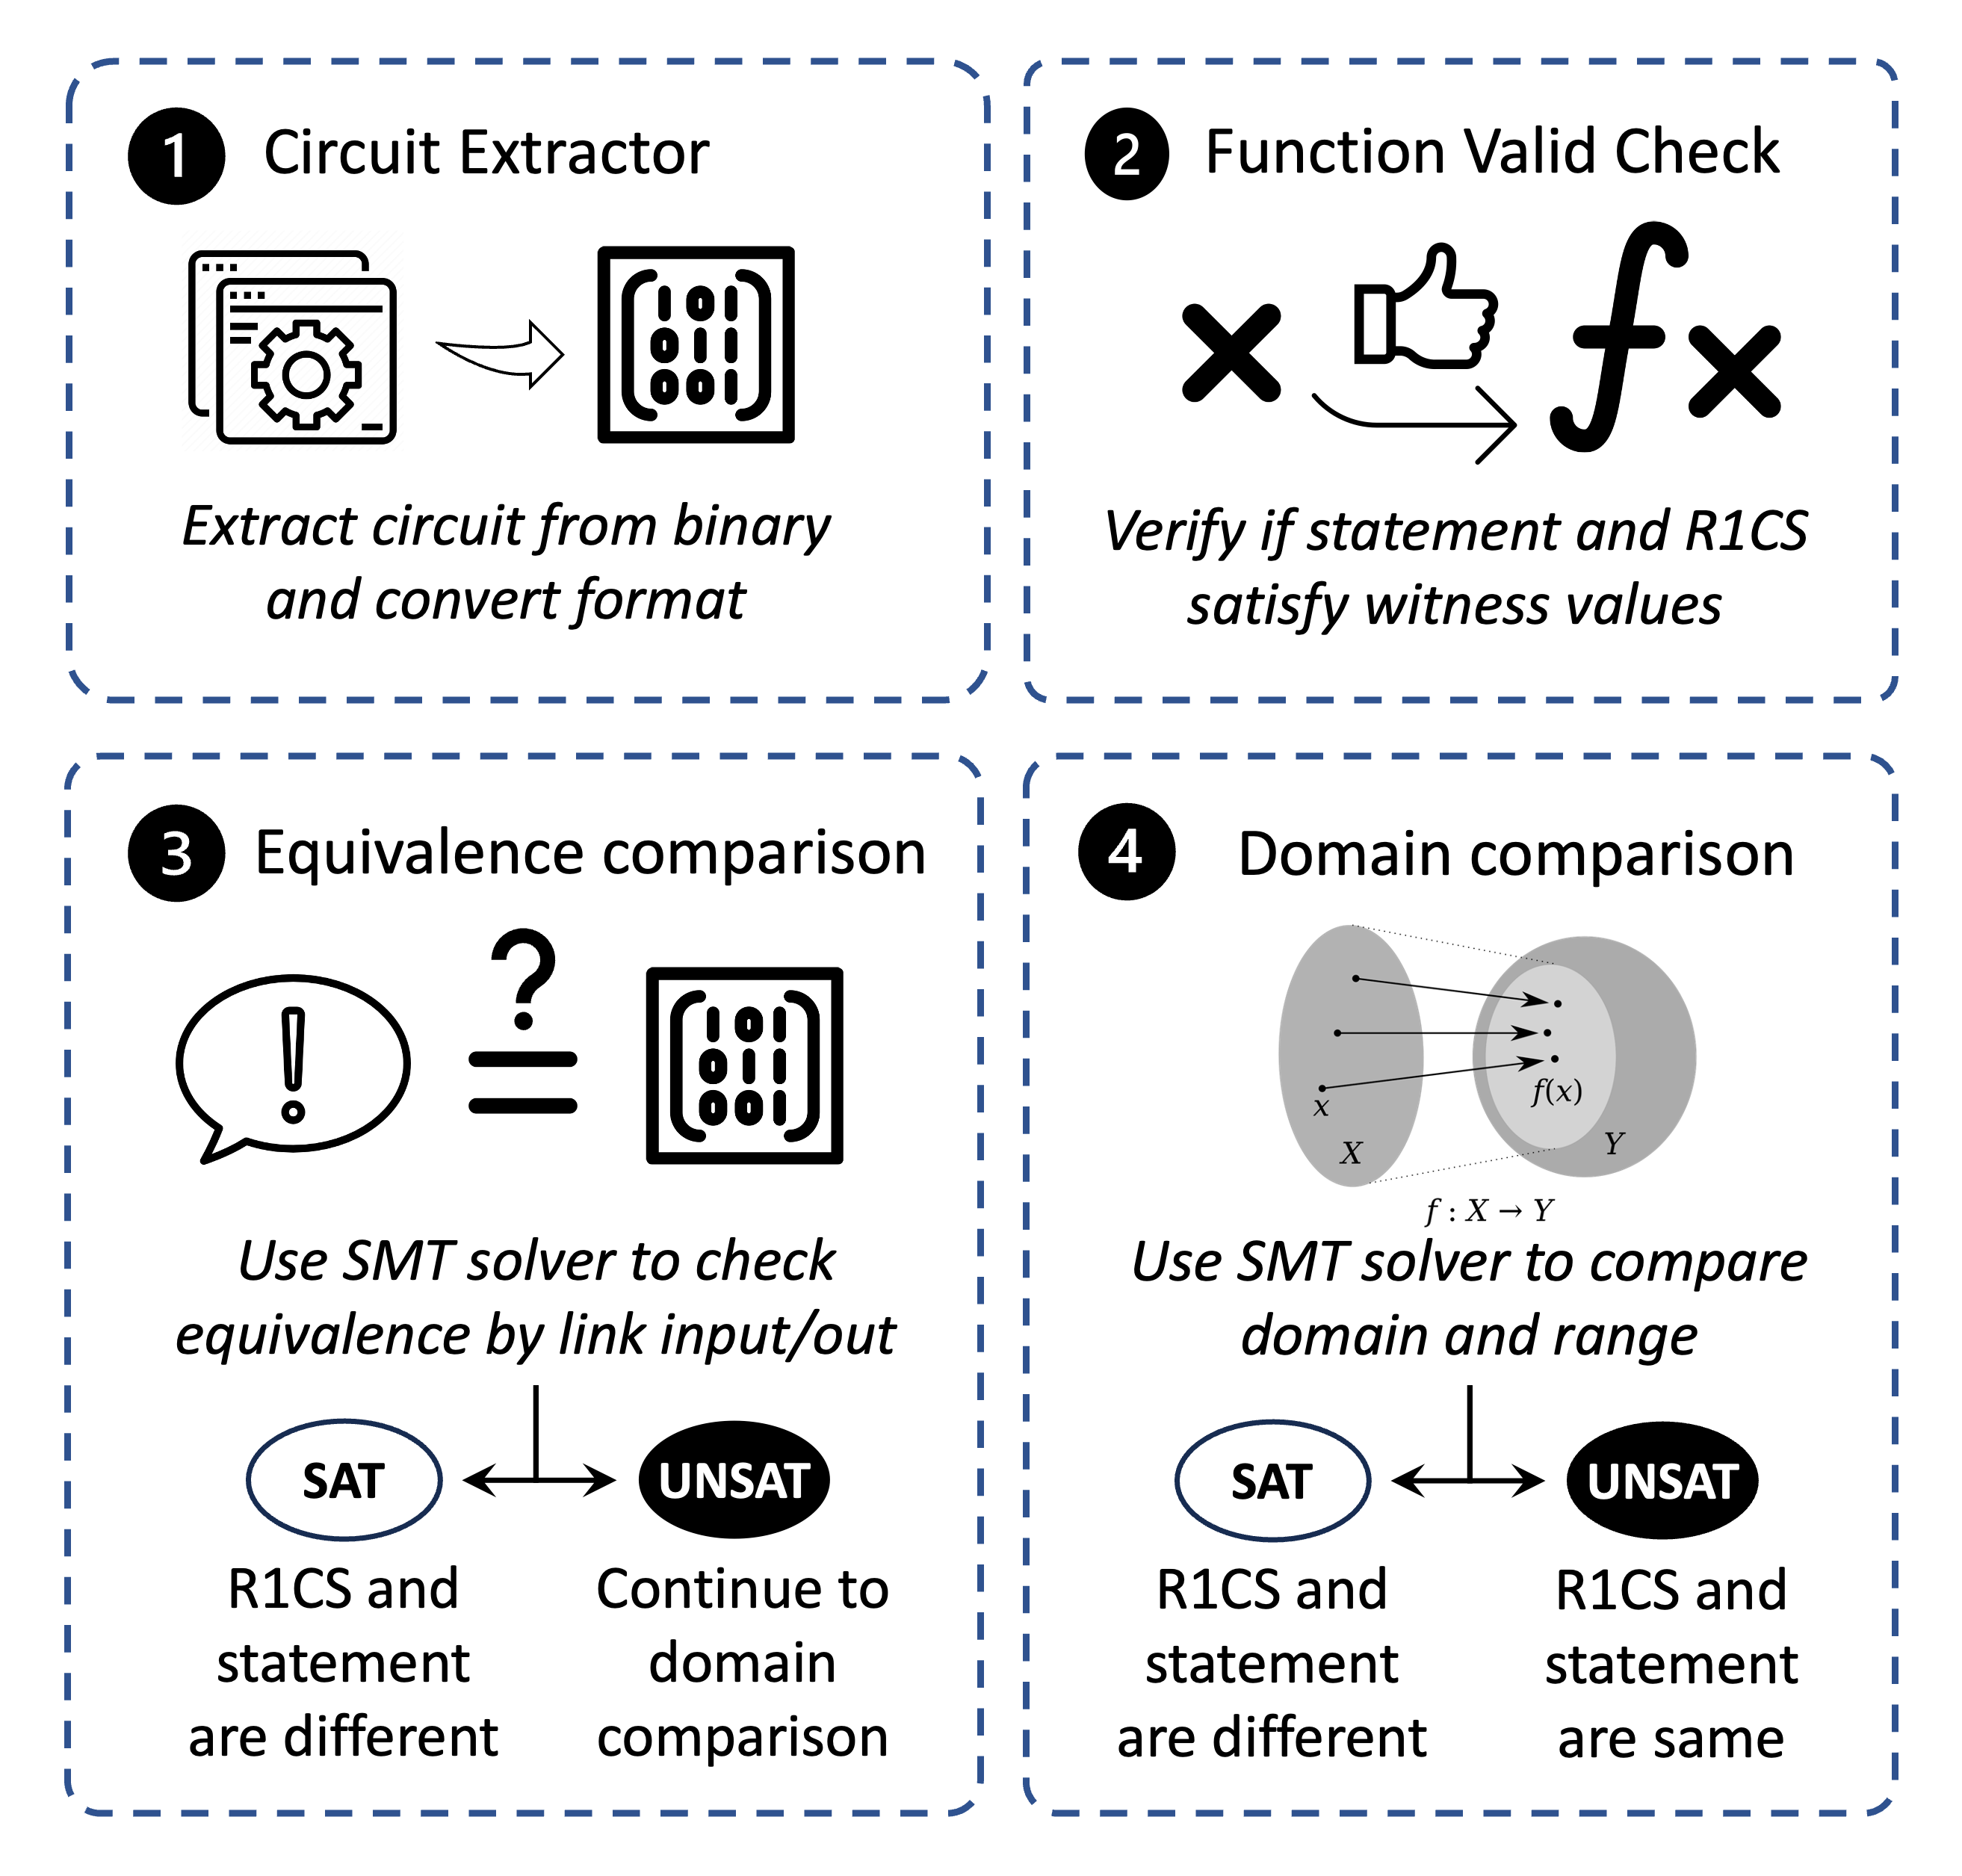
\includegraphics[height=2in]{ch-snarkprobe/figure/workflow_cc.png}
  \caption{\ConstraintChecker}
  \label{subfig:snarkprobe-workflow_cc}
\end{subfigure}
\hspace{-20pt}
\begin{subfigure}[b]{0.62\linewidth}
  \centering
  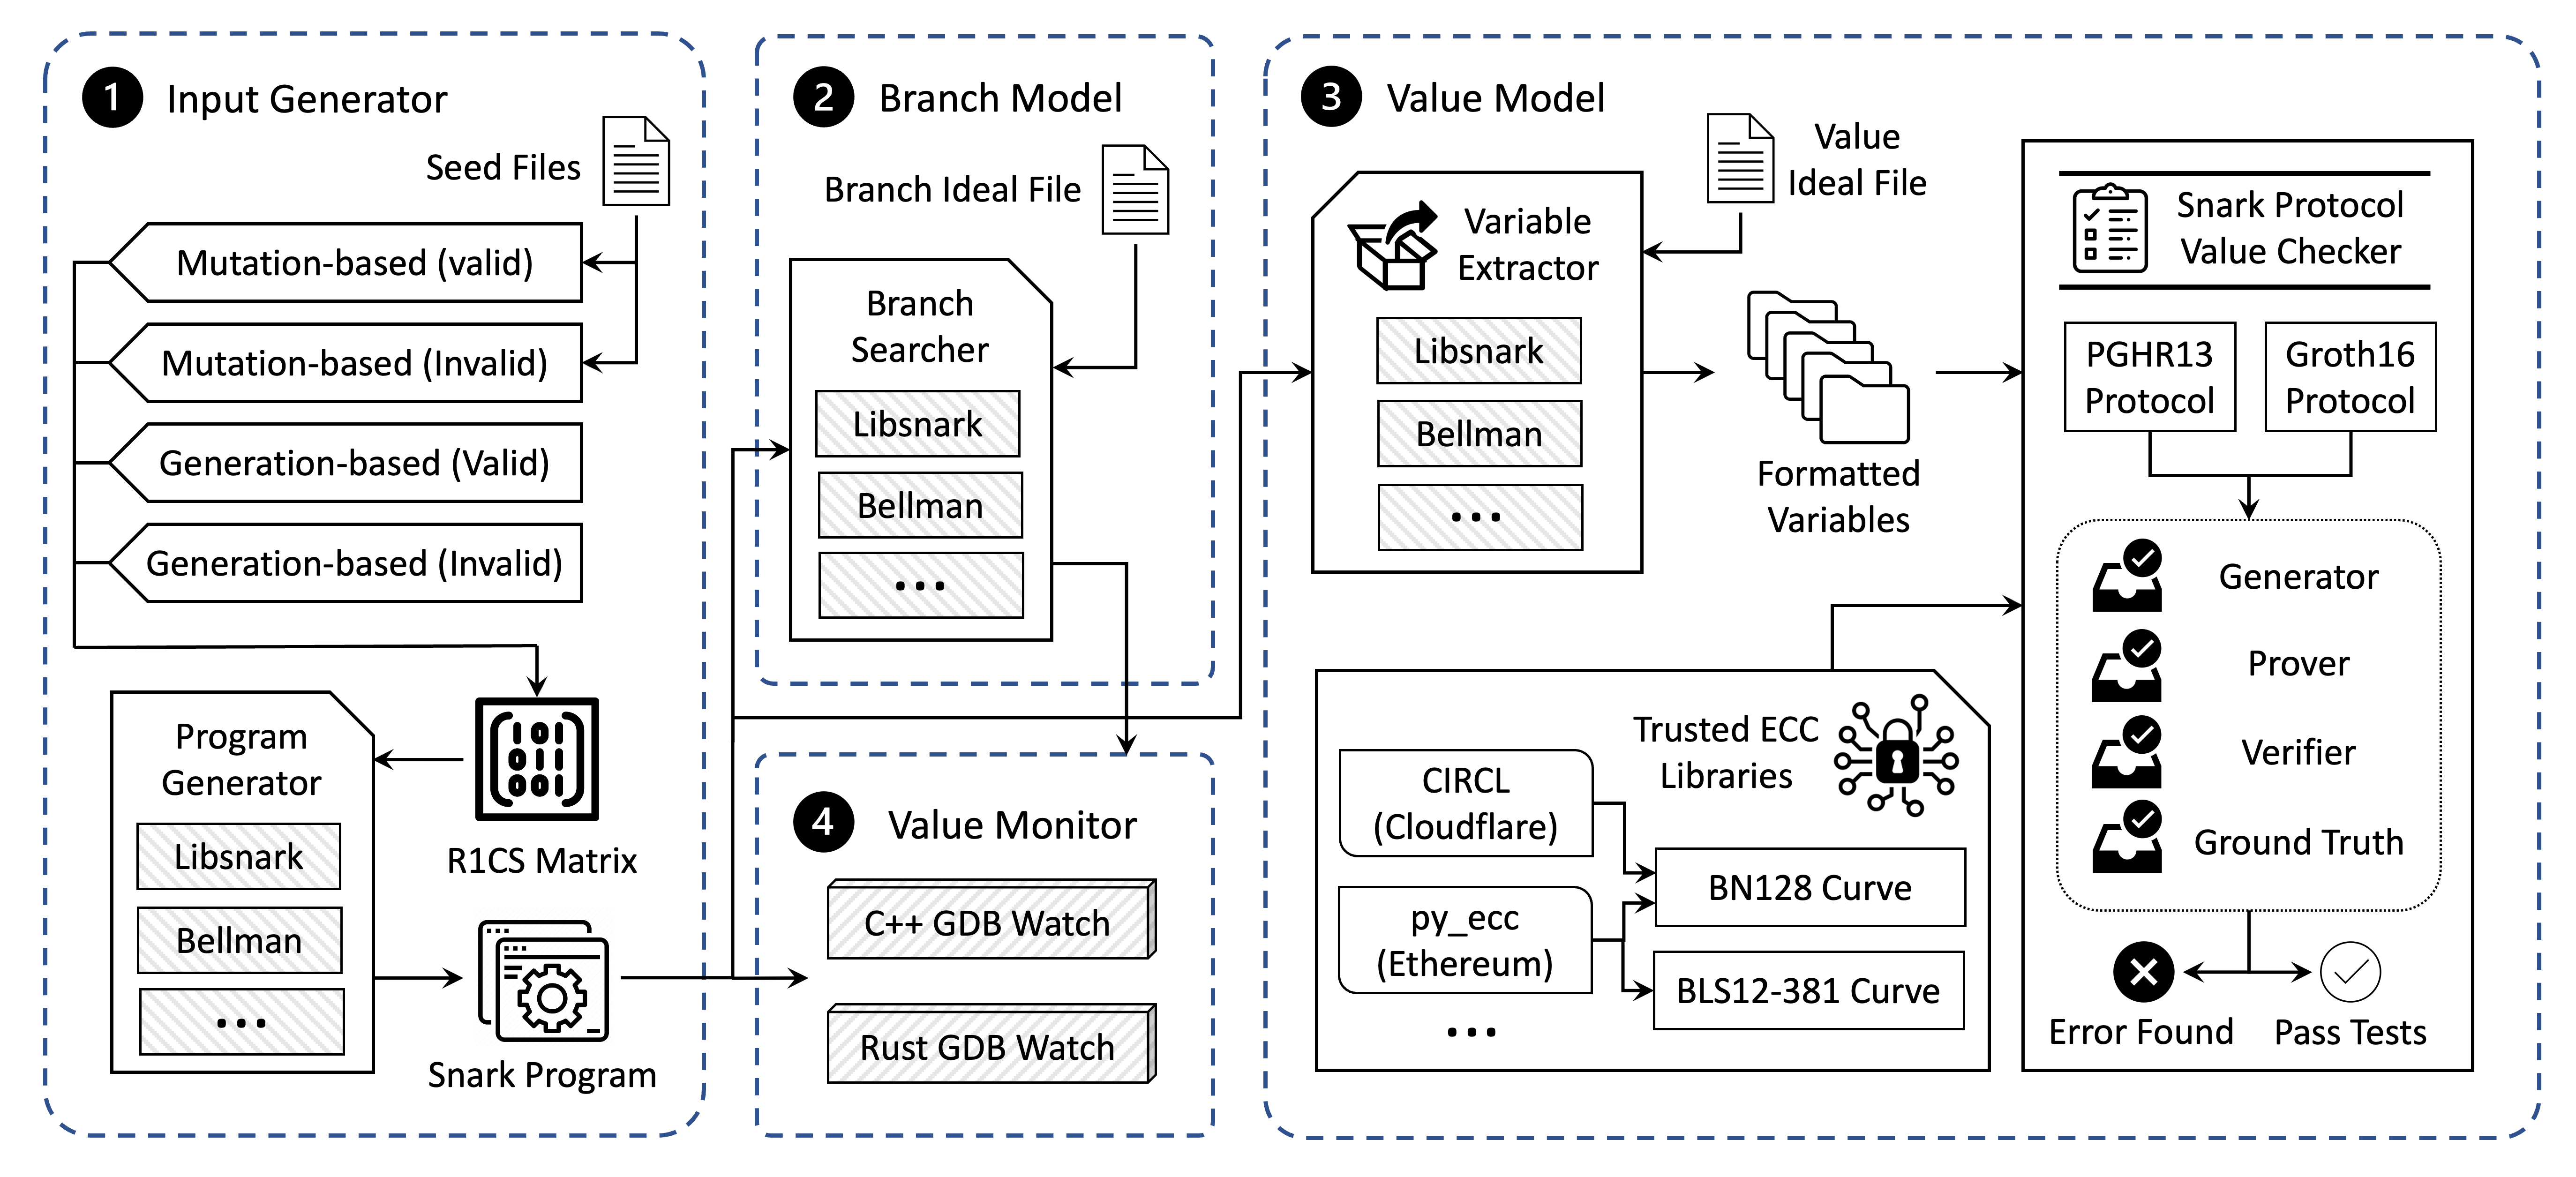
\includegraphics[height=2in]{ch-snarkprobe/figure/workflow_sf.png}
  \caption{\SnarkFuzzer}
  \label{subfig:snarkprobe-workflow_sf}
\end{subfigure}

\end{minipage}
\end{adjustbox}

\caption{Workflow of \tool. White boxes represent subcomponents universal for all zkSNARK libraries, forward diagonal stripes represent those designed for a specific library, and backward diagonal stripes represent those designed for a specific programming language.}
\label{fig:snarkprobe}
\end{figure}


\subsection{Workflow}

We now outline the workflow of running \tool, as well as establish terminology, before presenting the details and implementation in subsequent sections. \tool is composed of two broad sub-tools: the \ConstraintChecker and \SnarkFuzzer. These components can operate both independently of each other as well as in sequence, depending on what the user wishes to check.

Recall that at a high level, a \zksnark proof is generated in two main phases.  First (\textit{\circuitgen}), the user has a \textit{(proof) statement} that they wish to prove about, which requires converting this statement into a \textit{circuit} that the \zksnark protocol understands.
\textit{R1CS} is a specific form of this that we focus on in this work.  Second (\textit{\proofgen}), a \zksnark library takes the circuit (R1CS) as input and produces a proving key, verification key, and a \textit{proof}.


The first step verifies the consistency of a user-specified set of proof statement equations with the actual R1CS matrix used in the application, to ensure that the \circuitgen process generates the same proof as the developer states. The \ConstraintChecker uses an SMT solver to compare the input values, output values, domain, and range of the given statement equations with R1CS matrix to find any errors in the conversion. \autoref{subfig:snarkprobe-workflow_cc} shows the internal steps of the \ConstraintChecker, which we discuss in detail in \autoref{subsec:snarkprobe-constraintchecker}.


The second step checks the correctness of the library and \proofgen process. \autoref{subfig:snarkprobe-workflow_sf} shows the steps of \SnarkFuzzer, which we discuss in detail in \autoref{subsec:snarkprobe-snarkfuzzer}.
%%\fanyo{The \framework can evaluate the correctness of \zksnark library implementation.} 
First, the \inputgenerator produces an R1CS matrix (i.e., proof) using a variety of fuzzing techniques and compiles this into an executable proof program with the selected library, which serves as the input for the \branchmodel. Then, the \branchmodel investigates the visitation status for each branch during execution and provides feedback to the \inputgenerator to determine if another input is needed. This coverage feedback fuzzing helps improve the coverage rate of \SnarkFuzzer, which improves the chance of catching errors in the target library. Finally, the \valuemodel re-evaluates the protocol calculations to detect any potential cryptographic logic errors and looks for inconsistencies caused by unexpected value changes or implementation errors.
%%\fanyo{Since in the dynamic analysis, a single \framework evaluation cannot cover the entire library implementation. The \SnarkFuzzer will generates extra input seeds to execute multiple \framework check until the entire library has been fully evaluated.}

Together, these two components allow \tool to evaluate the end-to-end correctness and security of a specific implementation of a given proof statement for a given library (or to individually check different parts if desired).

Unlike standard fuzzers, \SnarkFuzzer can detect both software and \logicerror{s}.  We consider a \emph{software error} to be a bug or fault in the software that causes unintended behaviors or incorrect performance, such as crashing, overflow, or a system error.  A \emph{\logicerror}, on the other hand, is one that causes a program to produce an incorrect result due to errors in the cryptographic protocol implementation, such as incorrect mathematical operations or disregarding the specification. A \logicerror will not cause a software crash or raise an error message, making them much harder to detect.
For a basic example, in RSA, software errors might cause a program crash, but cryptographic logic errors are issues where the ciphertext value was not computed correctly ($m^e \mod N$ computed incorrectly) or too large a ciphertext was used (e.g., larger than the modulus).

%In general, \tool should be as automatic as possible, requiring little intervention from the developer.  However, there are still a few small manual pre-processing steps.
%First, to run the \ConstraintChecker, a user needs to indicate the proof statement.  After that, the \ConstraintChecker can run automatically to check the equivalence of the proof statement and circuit (R1CS).
%Second, before running \SnarkFuzzer, the user needs to manually create one ideal file containing the basic programming structure of the target library. However, this only needs to be done once ever per library that one wishes to test and could be done by anyone.
%We do not believe that these manual interventions require substantial cryptographic or zero-knowledge proof related expertise.

While we currently focus on R1CS-based zkSNARKS, we believe this high level design can be adapted without major changes to support additional (newer) types of proofs, particularly in the case of \SnarkFuzzer, which would largely only involve changing the input generation methodology and format.

\parhead{Why dynamic analysis?}
Dynamic analysis supports our goal of finding \logicerror{s} by allowing us to trace and extract real-time data and variable values, which we can then use to check for cryptographic protocol conformance and implementation errors.
It also allows us to easily support a number of different zkSNARK libraries written in different languages without the need for additional manual intervention, extensions, or program instrumentation by the user, making \tool flexible as well.
Our design choices mean that is easy to extend \tool to support new languages and libraries, without needing to investigate new instrumentation techniques or tools.

%In next two sections, we will go into more details and present how our tools detect errors in zk-SNARKs library. Section \ref{sec:design} introduces the design of the \ConstraintChecker and \SnarkFuzzer, and Section \ref{sec:implementation} demonstrates how we achieve our designs and the specific techniques we apply.

%\begin{figure*}[t]
  %\centering
  %\includegraphics[width=0.75\linewidth]{imgs/model.jpg}
	%\vspace*{-12pt}
  %\caption{Workflow in \SnarkFuzzer. White boxes represent subcomponents universal for all zkSNARK libraries, forward diagonal stripes represent those designed for a specific library, and backward diagonal stripes represent those designed for a specific programming language.}
  %\label{fig:snarkprobe-snarkfuzzer}
  %\vspace*{-8pt}
%\end{figure*}

%\parhead{Assumptions and Limitations.}
%Currently, \tool is a whitebox testing tool, and we assume that users have access to the program and library source code.  We leave extending \tool to work in a blackbox manner for future work.
%Also, \tool only works with R1CS-based zkSNARKs in our current implementation.  While we leave this for future work, we believe our high level design can be adapted without major changes to support additional (newer) types of proofs, particularly in the case of \SnarkFuzzer, which would largely only involve changing the input generation methodology and format.
%Finally, there are still a few small areas that require user intervention which we see as largely unavoidable in our current design, though we have sought to reduce these as much as possible and make them require the smallest amount of burden on or expertise from the user as possible.
%This includes the user indicating a proof statement for the \ConstraintChecker and the one-time per library creation of an ideal file containing the basic programming structure of the target library.

%\clg{Include some sort of short limitations paragraph.  For example, we require source code, there is still some manual effort needed (though a large amount of it only needs to be done once), etc.  Addressing these would be good avenues for future work.}
%\clg{Oh, we need to point out that this only works for R1CS based SNARKs, future work would then be to figure out how to adapt this to other, newer, types of SNARKs.}
%
%Even we remove most of the human affects in \tool, there are still a few manual interventions needed by our tools. \ConstraintChecker requires user allocating the public and private variables in correct order, or otherwise, \ConstraintChecker will raise a false alarm even the statement equations have been correctly converted into R1CS matrix. Meanwhile, developers also need to create the ideal files for \SnarkFuzzer when they want to test a new zk-SNARKs library or protocol. Creating ideal files is simply without requiring the understanding of high level zk-SNARKs knowledge. However, there is still some risks that developers may incorrectly implement the ideal files, and \SnarkFuzzer may have poor performance with ideal files that contains bias errors.
%
%\tool is a whitebox testing tool, and developers should have access to the program and library source code. A blackbox binary zk-SNARKs program cannot be examined by \ConstraintChecker and \SnarkFuzzer since our design can only handle the program compiled in debug mode. Also, \tool only works with rank-1 constraint system (R1CS) based on our current implementation, but this can be expanded in the future to adopt other, newer, types of zero knowledge proof without major revision in the high level design.